\section{Movimiento en dos dimensiones}
  \subsection{Vectores de posición, velocidad y aceleración}
    \PN En dos dimensiones, la posición de una partícula se indica mediante su vector de posición $\VB{r}$, que se
    dibuja desde el origen de algún sistema coordenado a la posición de la partícula en el plano xy.

    \begin{figure}[H]
    \centering
      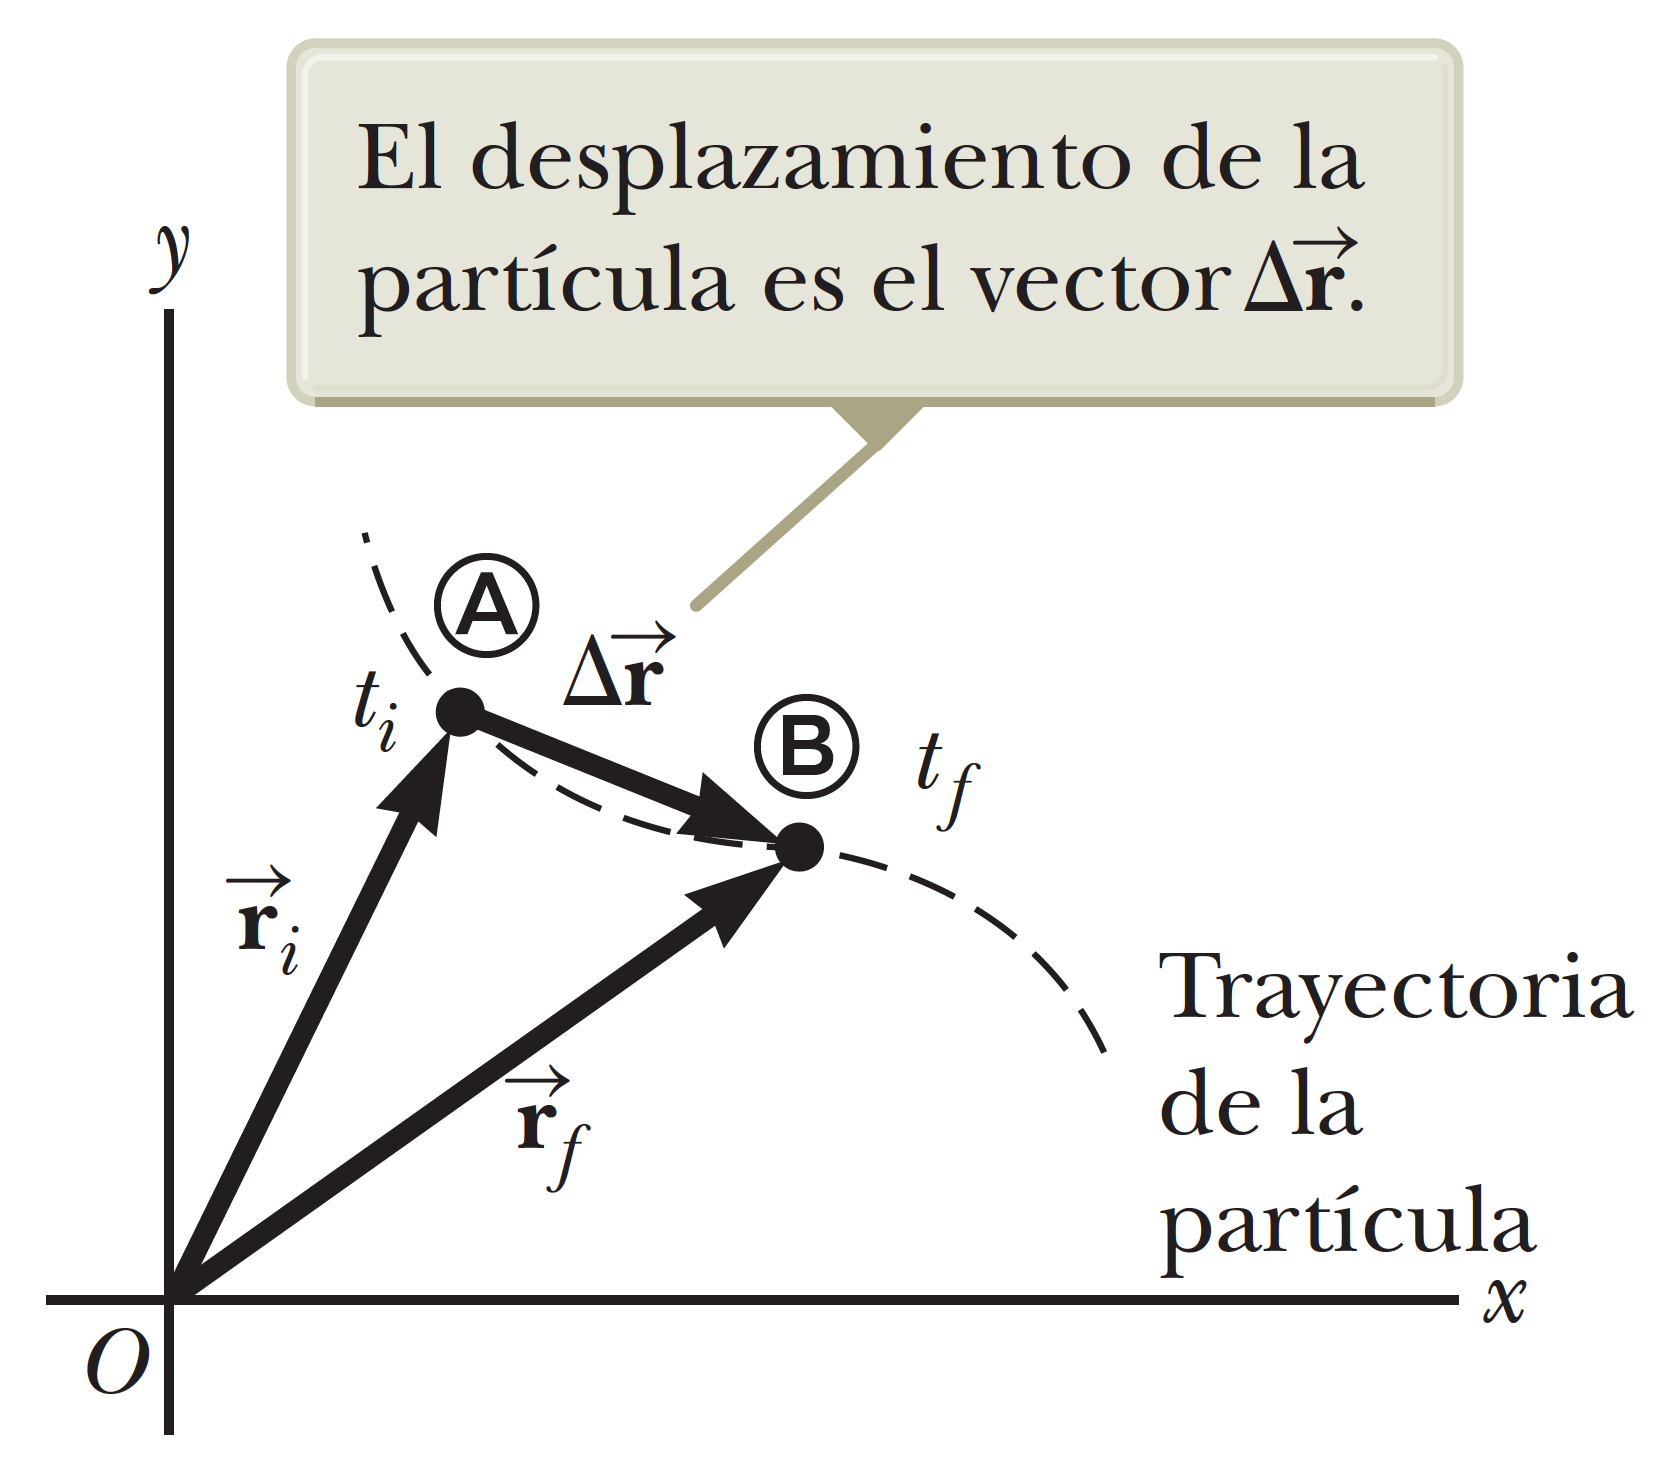
\includegraphics[width=0.4\textwidth]{1/figure_1}
      \caption{Una partícula que se mueve en el plano xy se ubica con el vector de posición $\VB{r}$, que se dibuja
      desde el origen hasta la partícula.}
    \end{figure}

    \begin{itemize}
      \item El \textbf{vector desplazamiento} $\VB{r}$ para una partícula se define como la diferencia entre su vector
      de posición final y su vector de posición inicial:
        \begin{equation*}
          \Delta \VB{r} = \VB{r}_{f} - \VB{r}_{i}
        \end{equation*}

      \item La \textbf{velocidad promedio} $\VB{v}_{prom}$ de una partícula durante el intervalo de tiempo $\Delta t$ se
      define como el desplazamiento de la partícula dividido entre el intervalo de tiempo:
        \begin{equation*}
          \VB{v}_{prom} \equiv \frac{\Delta \VB{r}}{\Delta t}
        \end{equation*}

      \item La \textbf{velocidad instantánea} $\VB{v}$ se define como el límite de la velocidad promedio $\Delta \VB{r}$
      / $\Delta t$ conforme $\Delta t$ tiende a cero:
        \begin{equation*}
          \VB{v} \equiv \lim_{\Delta t \rightarrow 0} \ \frac{\Delta \VB{r}}{\Delta t} = \frac{d \VB{r}}{dt}
        \end{equation*}

        \PN Esto es, la velocidad instantánea es igual a la derivada del vector de posición respecto del tiempo.

        \PN La magnitud del vector velocidad instantánea $ v = \abs{\VB{v}}$ de una partícula se llama \textit{rapidez}
        de la partícula, que es una cantidad escalar.

      \item La \textbf{aceleración promedio} $\VB{a}_{prom}$ de una partícula se define como el cambio en su vector
      velocidad instantánea $\VB{v}$ dividido entre el intervalo de tiempo $\Delta t$ durante el que ocurre dicho
      cambio:
        \begin{equation*}
          \VB{a}_{prom} \equiv \frac{\Delta \VB{v}}{\Delta t} = \frac{\VB{v}_{f} - \VB{v}_{i}}{t_{f} - t_{i}}
        \end{equation*}

      \item La \textbf{aceleración instantánea} $\VB{a}$ se define como el valor límite de la razón $\Delta \VB{v}$ /
      $\Delta t$ conforme $\Delta t$ tiende a cero:
        \begin{equation*}
          \VB{a} \equiv \frac{\Delta \VB{v}}{\Delta t} = \frac{d \VB{v}}{dt}
        \end{equation*}
    \end{itemize}

  \subsection{Movimiento en dos dimensiones con aceleración constante}
    \PN eEl movimiento en dos dimensiones se puede representar como dos movimientos independientes en cada una de las
    dos direcciones perpendiculares asociadas con los ejes x e y. Esto es: cualquier influencia en la dirección y no
    afecta el movimiento en la dirección x y viceversa.

    \PN El vector de posición para una partícula que se mueve en el plano xy se puede escribir
    \begin{equation*}
      \VB{r} = x \mathbf{\hat{i}} + y \mathbf{\hat{j}}
    \end{equation*}

    \PN donde x, y y $\VB{r}$ cambian con el tiempo a medida que la partícula se mueve mientras los vectores unitarios
    $\mathbf{\hat{i}}$ y $\mathbf{\hat{j}}$ permanecen constantes.

    \begin{itemize}
      \item \textbf{Vector velocidad:}
        \begin{equation*}
          \VB{v}_{f} = \VB{v}_{i} + \VB{a} t
        \end{equation*}

      \item \textbf{Vector de posición:}
        \begin{equation*}
          \VB{r}_{f} = \VB{r}_{i} + \VB{v}_{i} t + \frac{1}{2} \VB{a} t^{2}
        \end{equation*}
    \end{itemize}

  \subsection{Movimiento de un proyectil}
    \PN El \textbf{movimiento de proyectil} de un objeto es simple de analizar a partir de dos suposiciones:
    \begin{itemize}
      \item la aceleración de caída libre es constante en el intervalo de movimiento y se dirige hacia abajo
      \item el efecto de la resistencia del aire es despreciable
    \end{itemize}

    \PN La expresión para el vector de posición del proyectil como función del tiempo, siendo su aceleración la de la
    gravedad, $\VB{a} = \VB{g}$ es:
    \begin{equation*}
      \VB{r}_{f} = \VB{r}_{i} + \VB{v}_{i} t + \frac{1}{2} \VB{g} t^{2}
    \end{equation*}

    \PN donde las componentes x e y de la velocidad inicial del proyectil son:
    \begin{equation*}
      v_{xi} = v_{i} \cos(\theta) \qquad v_{yi} = v_{i} \sin(\theta)
    \end{equation*}

    \begin{figure}[H]
    \centering
      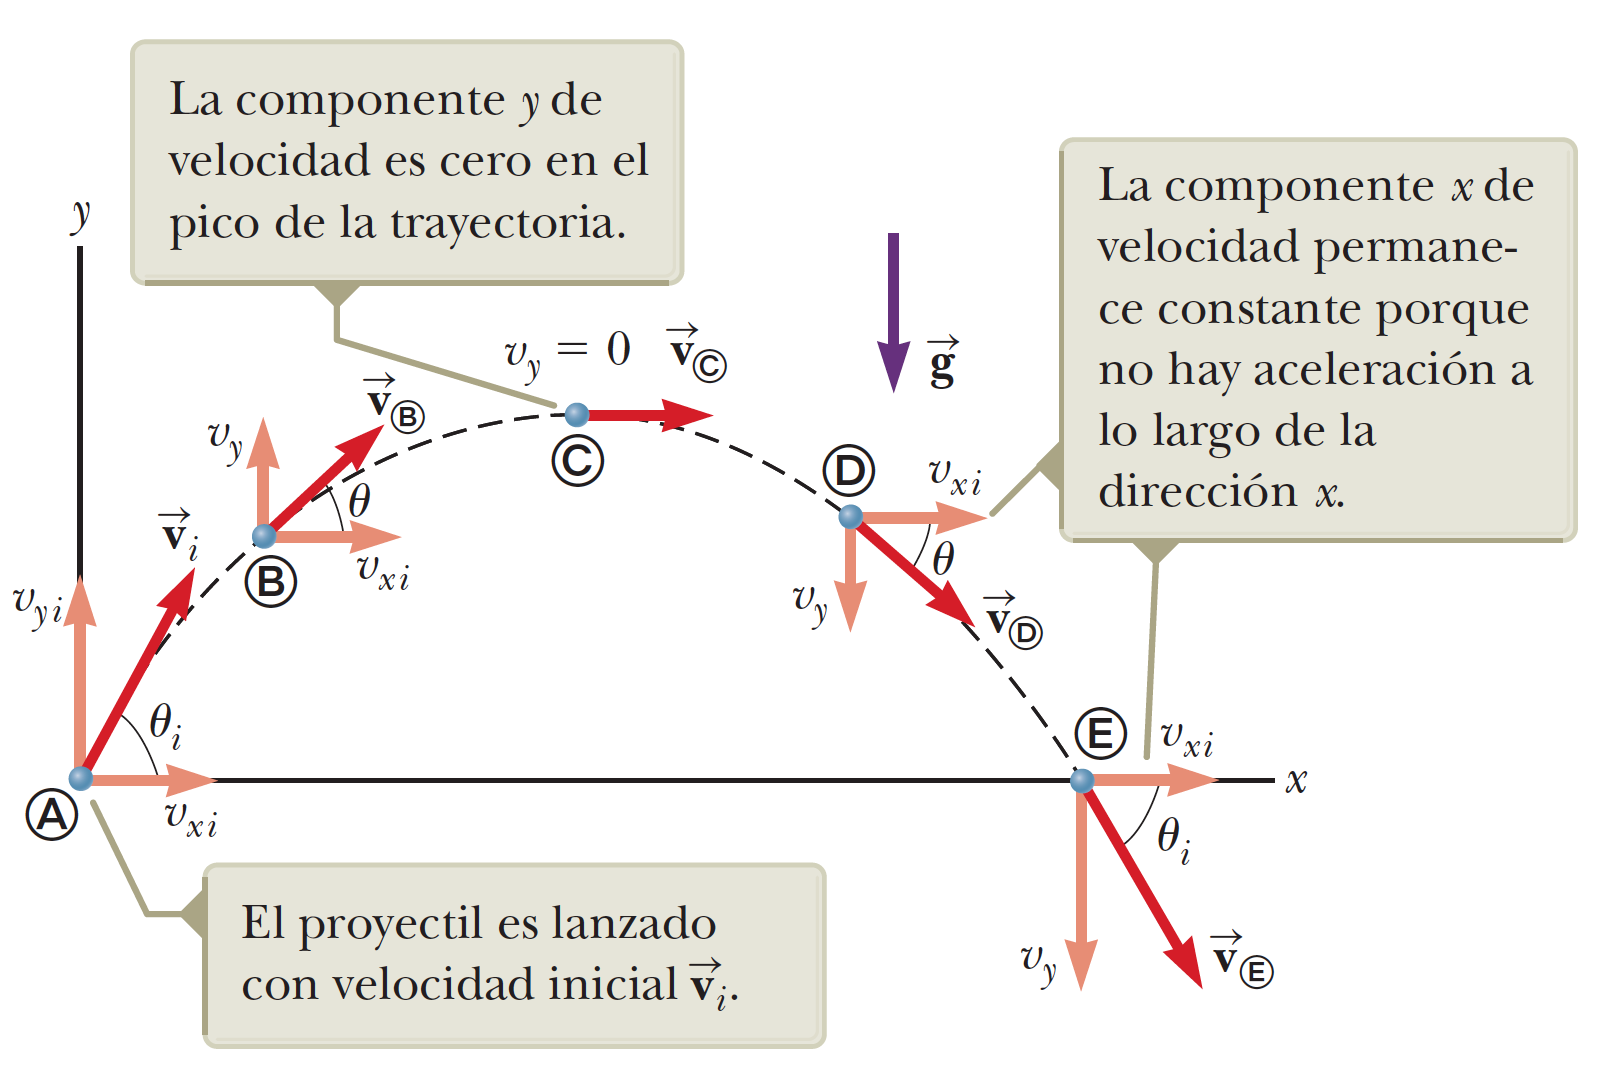
\includegraphics[width=0.6\textwidth]{1/figure_2}
      \caption{Trayectoria parabólica de un proyectil que sale del origen con velocidad $\VB{v}_{i}$. El vector
      velocidad $\VB{v}$ cambia con el tiempo tanto en magnitud como en dirección. Este cambio es el resultado de la
      aceleración $\VB{a} = \VB{g}$ en la dirección y negativa.}
    \end{figure}
